\chapter{Laser Characterization and Selection}
\thispagestyle{empty}

\section{Requirements for the Laser Source}

The performance of an interferometric measurement system strongly depends on the properties of the employed laser source. Since the displacement measurement in an interferometer is directly related to the laser wavelength, the laser must provide stable emission characteristics and sufficient beam quality. In addition, intensity fluctuations and beam distortions can reduce the visibility of the interference fringes and therefore decrease the measurement accuracy \prismcite{28}. 

A total of six different laser sources were characterized experimentally. The characterization included wavelength measurements using a spectrometer, beam profile measurements for the determination of the beam quality factor \(M^2\), and intensity stability measurements using a power meter.

\section{Wavelength Measurements}

The wavelengths of the investigated laser sources were measured using a spectrometer. The laser beam was first redirected using a mirror and then coupled into an optical fiber connected to the spectrometer using a convex CaF\(_2\) lens with a focal length of 50 mm. The setup is shown in Figure~\ref{fig:spectrometer_setup}.

\begin{figure}[htbp]
    \centering
    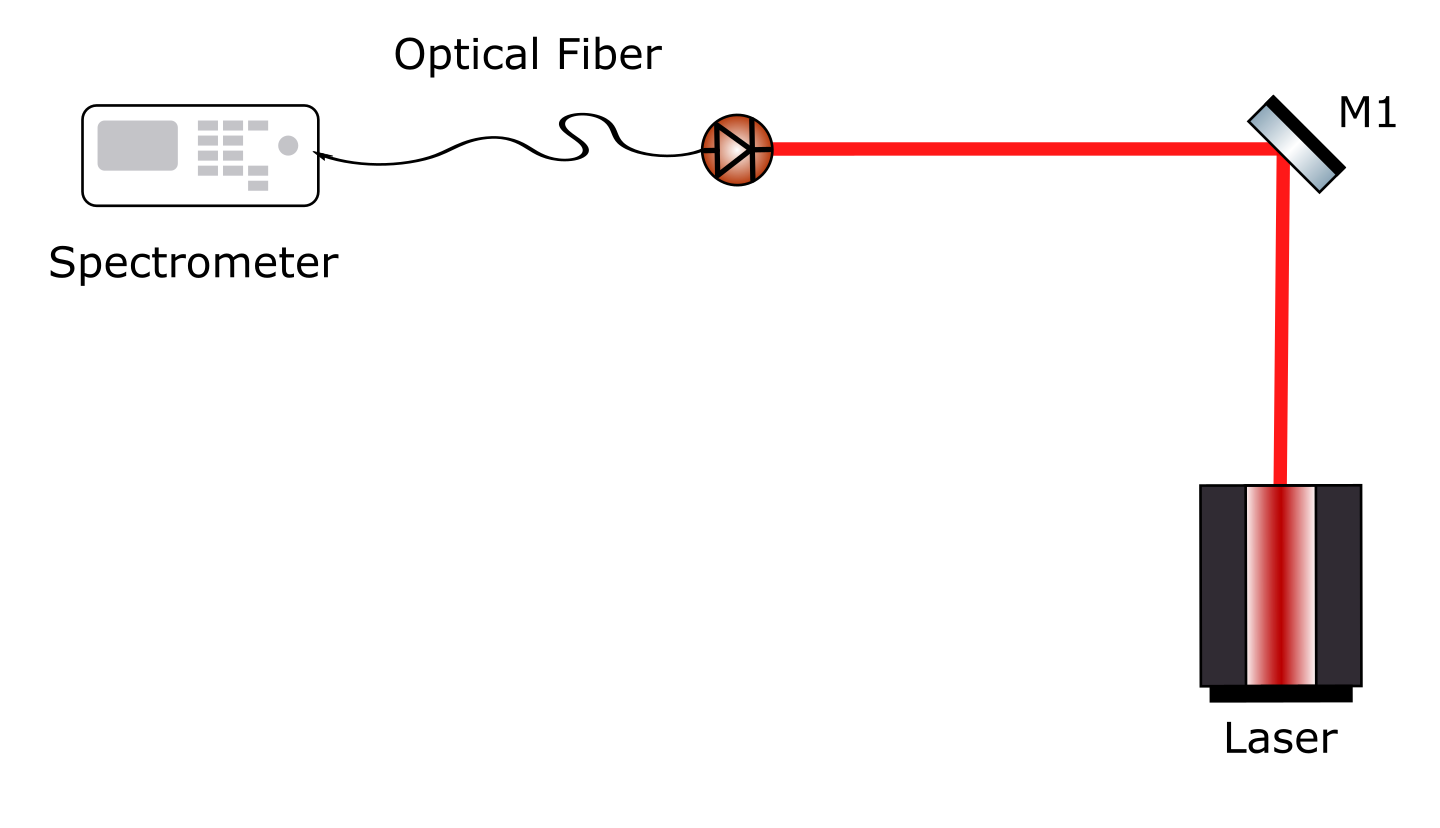
\includegraphics[width=0.55\linewidth]{figures/wavelengthmeasureincscape.png}
    \caption{Experimental setup and schematic representation of the wavelength measurements with the spectrometer. In the schematic, M1 denotes the mirror.}
    \label{fig:spectrometer_setup}
\end{figure}

The wavelengths of the laser sources were measured using an Ocean Optics SR6VN500-10 spectrometer covering the spectral range from 300 nm to 1100 nm. Due to the high optical power of the laser sources, the detector signal exceeded the dynamic range of the OceanView acquisition software, leading to saturation. Therefore absorptive neutral density filters were inserted into the beam path between the mirror and the spectrometer input.

Additionally, for every measurement a background spectrum without laser illumination was recorded. This background signal was subtracted from the measured spectra in order to reduce detector noise.

The measured peak wavelengths of the investigated laser sources are summarized in Table~\ref{tab:wavelengths}. The corresponding background-corrected spectra are shown in Figure~\ref{fig:all_corrected_lasers}.

\begin{table}[htbp]
\centering
\caption{Measured peak wavelengths of the investigated laser sources.}
\label{tab:wavelengths}
\begin{tabular}{lc}
\hline
Laser Source & Peak Wavelength (nm) \\
\hline
Thorlabs CPS780S & 787.32 \\
Uniphase 1023P & 631.81 \\
Uniphase 1103P 1177761 & 631.81 \\
Uniphase 1103P 1108380 & 632.01 \\
Uniphase 1122P & 632.21 \\
Uniphase 1507P & 634.82 \\
\hline
\end{tabular}
\end{table}

\begin{figure}[htbp]
    \centering
    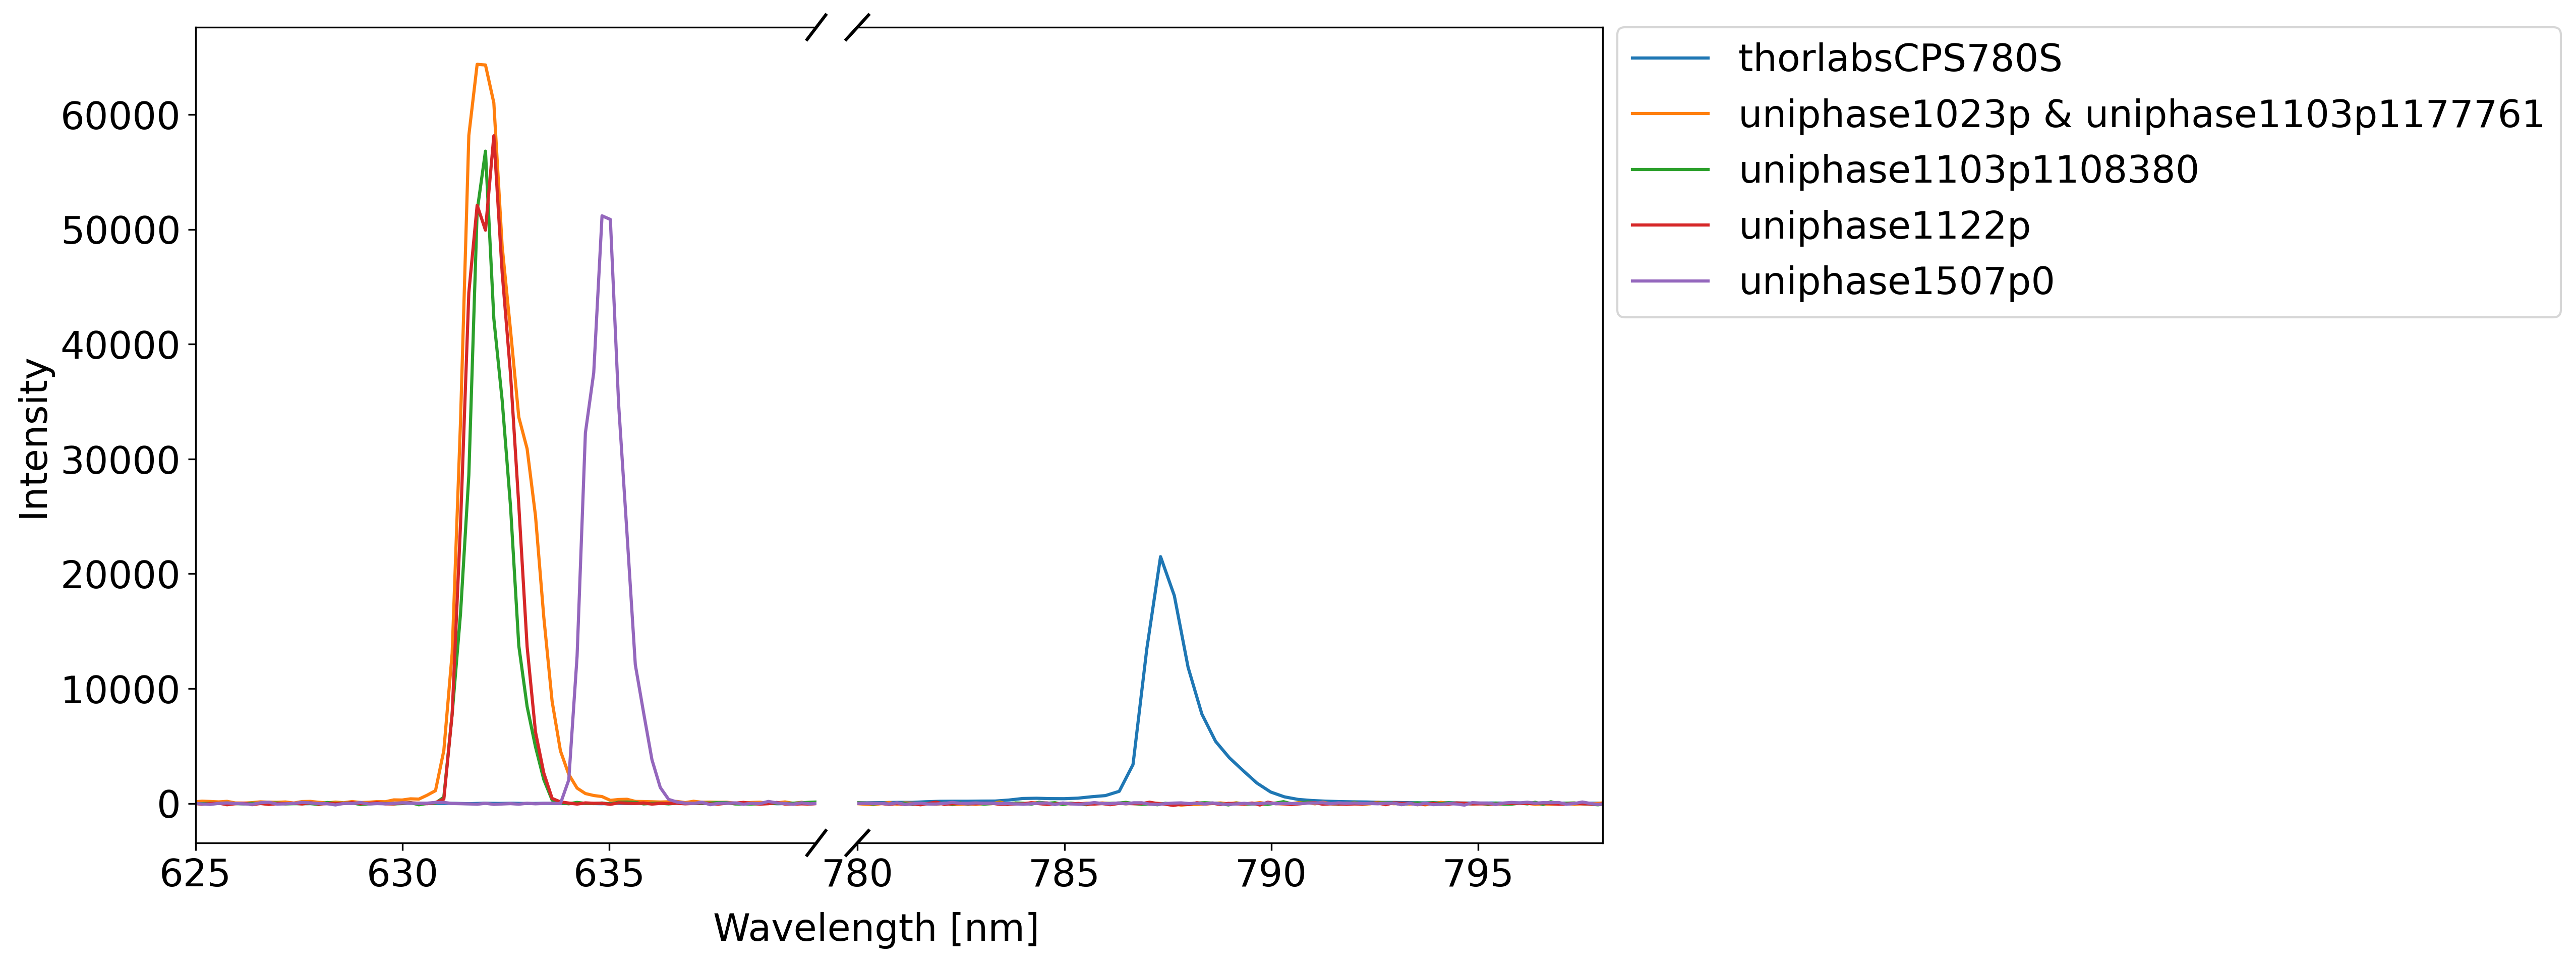
\includegraphics[width=\linewidth]{figures/all_corrected_lasers.png}
    \caption{Background-corrected spectra of the investigated laser sources used to determine the peak emission wavelengths. The spectra of the Uniphase 1023P and Uniphase 1103P (1177761) were identical, apart from severe detector saturation in the latter. Therefore, the unsaturated spectrum is used to represent both sources. Although minor saturation occurred for some spectra (such as the Uniphase 1507P and 1023P), the peak emission wavelengths could still be determined accurately.}
    \label{fig:all_corrected_lasers}
\end{figure}

The Uniphase HeNe laser sources emitted wavelengths close to the expected wavelength of approximately 632.8 nm. The measured deviations are likely caused by differences in the laser cavity, the gas composition, and the gas pressure but could also originate from spectrometer-calibration or resolution. The Thorlabs Diode Laser emitted a wavelength of 787.3 nm.

\section{Beam Profile Measurements and Determination of Beam Quality Factor}

As introduced in Chapter~\ref{chap:theoretical_background}, another key parameter for characterizing laser beams is the beam quality factor \(M^2\). In this work, \(M^2\) was determined using a RayCi beam profiling camera. For the measurements, the laser beam was redirected by a mirror and focused using a lens with a focal length of \(75\,\mathrm{mm}\). The experimental setup is shown in Figure~\ref{fig:beamprofile_setup}.

\begin{figure}[htbp]
    \centering
    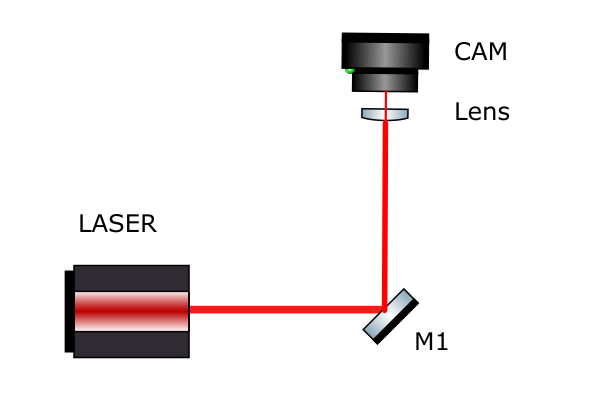
\includegraphics[width=0.45\linewidth]{figures/Beamqualityincscape.png}
    \caption{Experimental setup and schematic representation of the beam profile measurements with the RayCi beam profiling camera. In the schematic, M1 denotes the mirror and CAM denotes the RayCi beam profiling camera.}
    \label{fig:beamprofile_setup}
\end{figure}

Since the optical power of several laser sources exceeded the permissible detector range of the camera sensor, absorptive neutral density filters were inserted into the beam path to prevent detector saturation.

\subsection{Beam Diameter Measurements}

The beam profile measurements were performed using the RayCi software. For each laser source, the beam diameter was measured along the propagation direction in steps of 1 mm. The beam diameters were determined by the RayCi software separately for both transverse beam axes using the D4\(\sigma\) method in accordance with ISO 11146 \prismcite{40}.

The D4\(\sigma\) method defines the beam diameter based on the second moments of the measured intensity distribution and is particularly suitable for the characterization of non-ideal laser beams \prismcite{41}. The resulting beam diameters were recorded as a function of the propagation distance and subsequently exported for further analysis. 

\subsection{Determination of the Beam Quality Factor}

While the RayCi software provides beam diameter measurements, it does not directly calculate the beam quality factor \(M^2\). Therefore, the exported D4\(\sigma\) beam diameters were evaluated using a dedicated analysis program provided by Dr. Sergio Revuelta.

The program performs a nonlinear least-squares fit of the measured beam radii to the propagation model of a real Gaussian beam according to ISO 11146. The beam quality factor is defined as

\begin{equation}
M^2 = \frac{\pi w_0 \theta}{\lambda},
\end{equation}

where \(w_0\) is the beam waist radius, \(\theta\) is the far-field divergence angle, and \(\lambda\) is the laser wavelength \prismcite{42}.

Using the measured beam radii as a function of propagation distance, the fitting software determines the beam waist radius \(w_0\), the waist position \(z_0\), the divergence angle \(\theta\), the Rayleigh range \(z_R\), and the corresponding beam quality factor \(M^2\) independently for both transverse beam axes. The fitted propagation curves were compared with the measured data to assess the fit quality and the applicability of the Gaussian beam propagation model. To ensure reliable \(M^2\) determination, ISO 11146 requires measurement points both near the beam waist and in the far field. 

Figure~\ref{fig:m2fit_combined} shows the combined measured beam radii of all beams and the corresponding fitted propagation curves. The minimum of each fitted curve indicates the beam waist position, while the slope in the far field determines the beam divergence. Again, all Uniphase HeNe lasers exhibited very similar propagation curves and \(M^2\) values, whereas the Thorlabs diode laser showed a significantly higher \(M^2\) value, indicating poorer beam quality.

\begin{figure}[htbp]
    \centering
    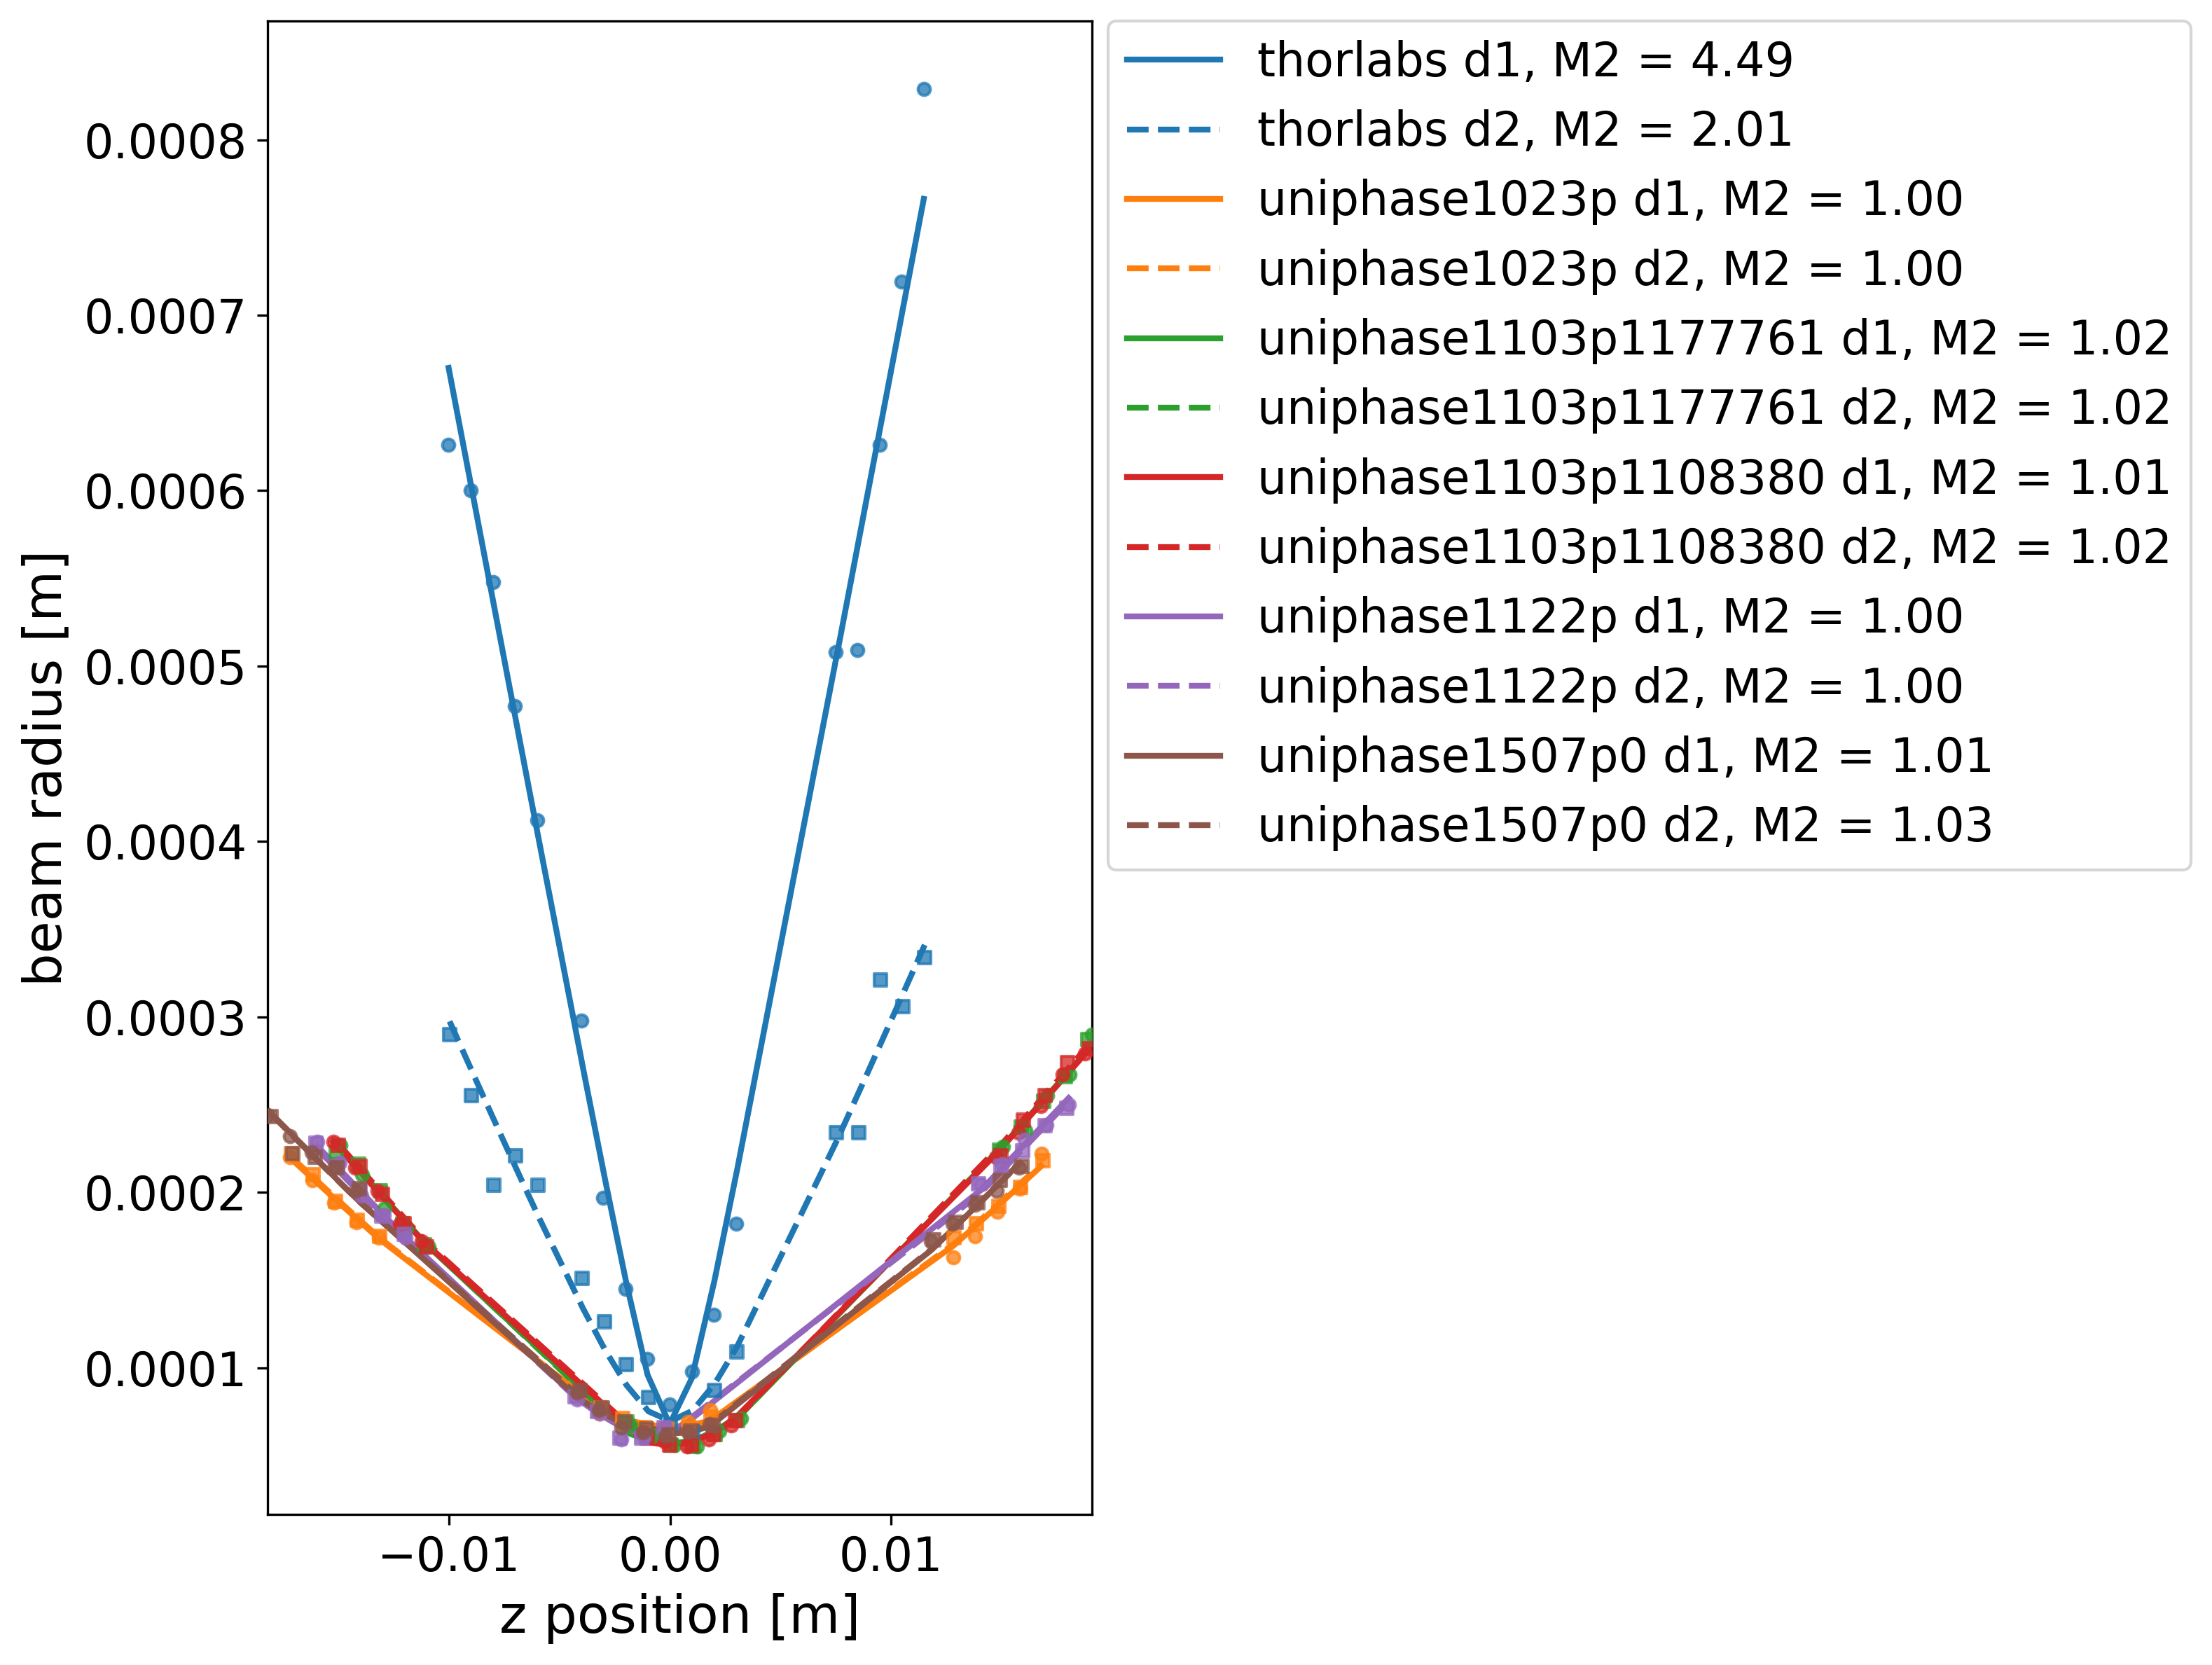
\includegraphics[width=0.8\linewidth]{figures/all_lasers_combined_fit.png}
    \caption{Measured beam radii and fitted beam propagation curves. The beam propagation model was fitted independently for both transverse beam axes. Discrete data points represent the measured values, while lines indicate the corresponding fits.}
    \label{fig:m2fit_combined}
\end{figure}


The resulting beam propagation parameters for all investigated laser sources are summarized in Table~\ref{tab:m2results}.

\begin{table}[htbp]
    \centering
    \caption{Measured beam propagation parameters of the investigated laser sources.}
    \label{tab:m2results}
    \begin{tabular}{lcccc}
        \hline
        Laser Source & \(M_x^2\) & \(M_y^2\) & Waist Radius x (\(\mu\)m) & Waist Radius y (\(\mu\)m) \\
        \hline
        Thorlabs CPS780S & 4.49 & 2.01 & 67.7 & 69.5 \\
        Uniphase 1023P & 1.00 & 1.00 & 66.2 & 65.8 \\
        Uniphase 1103P 1177761
         & 1.02 & 1.02 & 56.5 & 56.6 \\
        Uniphase 1103P 1108380 & 1.01 & 1.02 & 56.0 & 55.6 \\
        Uniphase 1122P & 1.00 & 1.00 & 59.0 & 59.3 \\
        Uniphase 1507P & 1.01 & 1.03 & 62.2 & 63.9 \\
        \hline
    \end{tabular}
\end{table}


 
 \section{Intensity Stability Measurements}

The temporal intensity stability of the laser sources was investigated using an Ophir Vega power meter. The laser beam was redirected using a mirror and directed onto the power meter detector. The experimental setup is shown in Figure~\ref{fig:powermeter_setup}.

\begin{figure}[htbp]
    \centering
    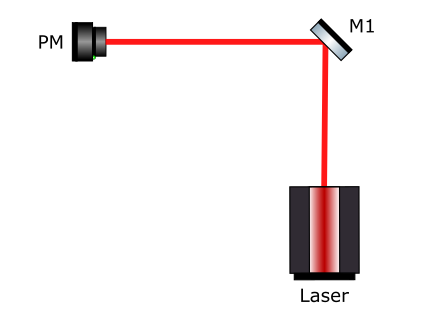
\includegraphics[width=0.55\linewidth]{figures/intensitystabiincscape.png}
    \caption{Experimental setup and schematic representation of the intensity stability measurements with the Ophir Vega power meter. In the schematic, M1 denotes the mirror and PM denotes the power meter.}
    \label{fig:powermeter_setup}
\end{figure}

For each laser source, the optical power was recorded over a time interval of approximately 600 s. The measured signals were analyzed with respect to their mean optical power, standard deviation, and signal-to-noise ratio (SNR). Figure~\ref{fig:intensitycomparison} shows the recorded power measurements of all investigated laser sources.

\begin{figure}[htbp]
    \centering
    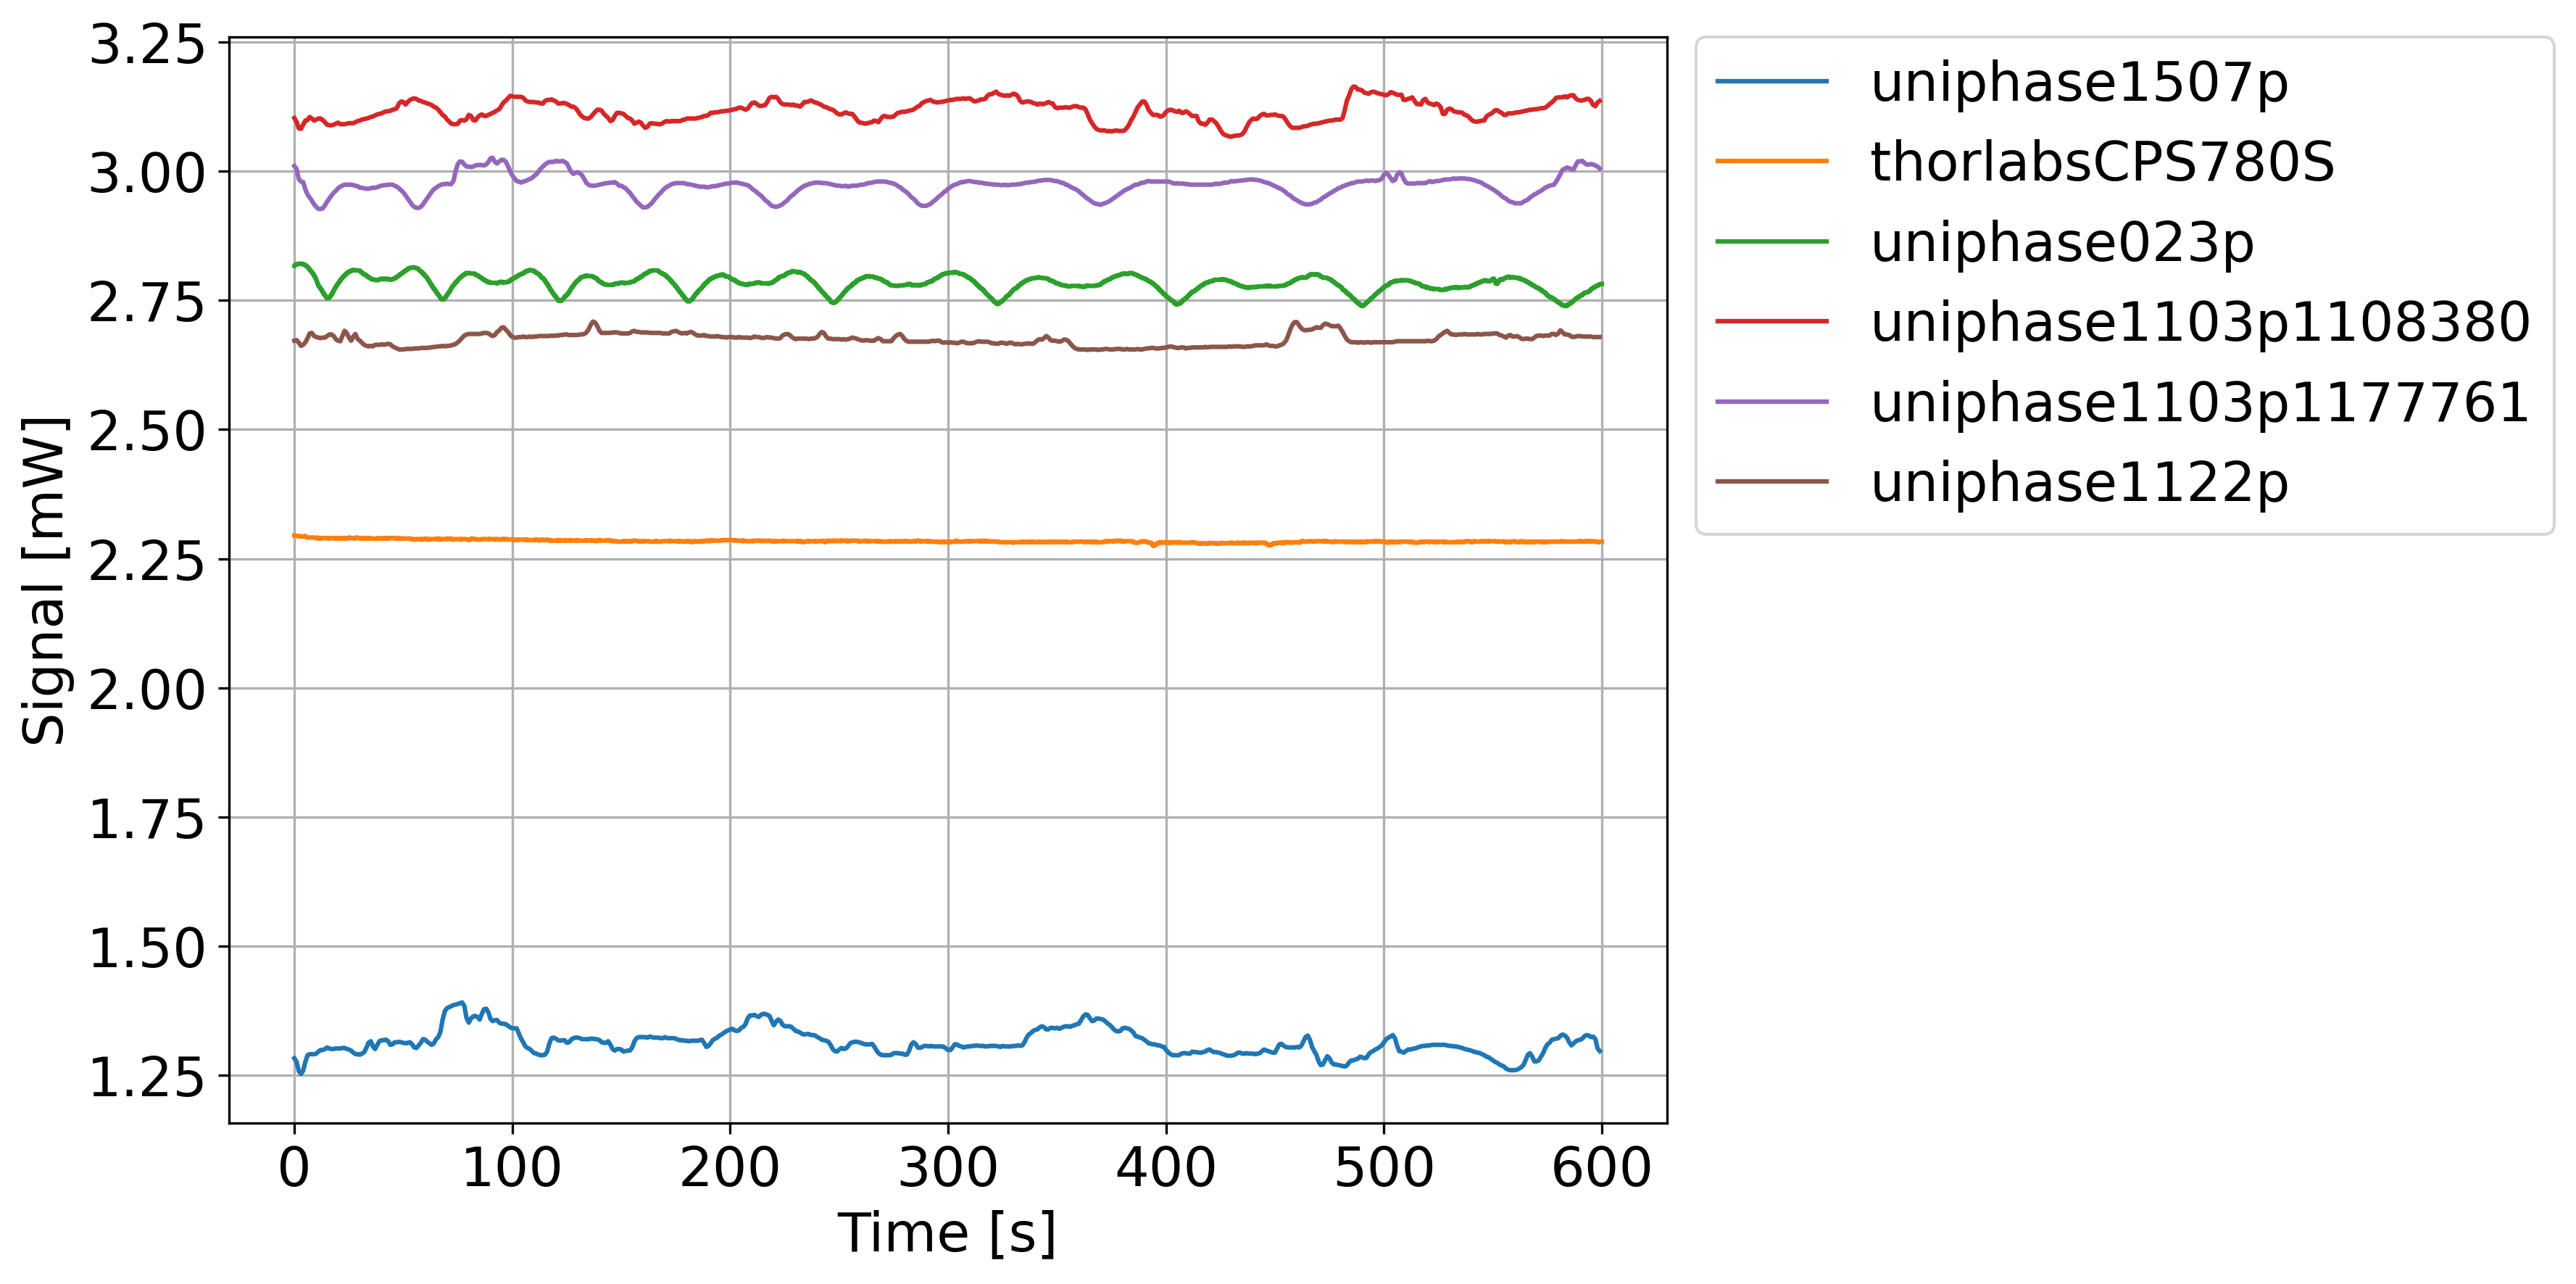
\includegraphics[width=0.75\linewidth]{figures/intensitycomparison.png}
    \caption{Comparison of the measured laser intensities over time.}
    \label{fig:intensitycomparison}
\end{figure}

The calculated SNR values are summarized in Table~\ref{tab:snrresults}.

\begin{table}[htbp]

\centering

\caption{Measured signal-to-noise ratios of the investigated laser sources.}

\label{tab:snrresults}

\begin{tabular}{lc}

\hline

Laser Source & SNR \\

\hline

Uniphase 1507P & 53.11 \\

Thorlabs CPS780S & 836.51 \\

Uniphase 1023P & 170.13 \\

Uniphase 1103P 1108380 & 155.98 \\

Uniphase 1103P 1177761 & 146.00 \\

Uniphase 1122P & 231.11 \\

\hline

\end{tabular}

\end{table}

The Thorlabs laser source exhibited the highest signal-to-noise ratio and the smallest intensity fluctuations over time. All of the Uniphase laser sources showed periodic fluctuations and increased noise contributions, which negatively affect interferometric fringe stability.

\section{Selection of the Final Laser Source}
Based on the wavelength measurements, beam profile analysis, and intensity stability measurements, the investigated laser sources were evaluated with respect to their suitability for interferometric displacement measurements.

Among the tested laser sources, the Thorlabs laser exhibited the highest intensity stability and the best signal-to-noise ratio. Although its operating wavelength differs from that of the investigated HeNe lasers, this does not constitute a disadvantage for the intended interferometric measurements, as the measurement principle itself is independent of the absolute wavelength, provided that the wavelength is accurately known.

The beam quality analysis revealed that the Thorlabs laser exhibited the highest \(M^2\) value among the investigated sources, indicating a greater deviation from an ideal Gaussian beam. However, for the Michelson interferometer developed in this work, intensity stability and signal quality were found to be more critical than achieving a near-ideal Gaussian beam profile, since the fringe detection algorithm analyzes only the central part of the beam, making the overall beam shape of secondary importance. In contrast, intensity fluctuations may cause incorrect fringe detection, directly affecting the accuracy of the displacement measurement. Consequently, the superior stability characteristics of the Thorlabs laser outweighed its reduced beam quality, and it was therefore selected as the light source for all subsequent interferometric measurements.